\chapter{Đại cương về tập hợp}

\section{Tập hợp}

Một tập hợp (set) bao gồm các phần tử khác nhau. Để biểu diễn tập hợp
ta có hai cách.

\begin{enumerate}
    \item Liệt kê. Ví dụ $A = \{ 1, 2, 3, 4 \}$, $B = \{ a, b , c \}$
    \item Sử dụng tính chất đặc trưng. Ví dụ $A = \{ a \in \NN^*, a < 5 \}$.
\end{enumerate}

Ở đây hai cách biểu diễn tập hợp $A$ là giống nhau.

\begin{definition}[Tập hợp rỗng]
    Tập hợp rỗng không chứa phần tử nào, ký hiệu là $\emptyset$.
\end{definition}

\begin{definition}[Tập hợp con]
    Xét tập hợp $A$. Tập hợp $B$ được gọi là \textbf{tập hợp con} của tập $A$
    nếu mọi phần tử của $B$ đều nằm trong $A$. Nói cách khác với mọi $b \in B$ thì
    $b \in A$. Ta ký hiệu $B \subset A$.
\end{definition}

Như vậy, \textit{tập hợp rỗng là con của mọi tập hợp}.

Dễ thấy rằng mọi tập hợp là tập hợp con của chính nó. Do đó tập con này được gọi là
tập con tầm thường (trivial subset). Để ký hiệu một tập con có thể bằng tập chứa nó
ta viết $B \subseteq A$. Trong trường hợp $B$ là tập con của $A$ nhưng không bằng 
$A$ ta có thể viết $B \subsetneq A$.

\section{Toán tử trên tập hợp}

Chúng ta xem xét 3 toán tử cơ bản trên tập hợp là \textit{giao}, \textit{hợp}
và \textit{hiệu} của hai tập hợp. Để biểu diễn các toán tử này ta có thể dùng 
biểu đồ Venn.

\begin{definition}[Giao của hai tập hợp]
    Giao của hai tập hợp $A$ và $B$ là tập hợp các phần tử thuộc cả $A$ và $B$.
    \begin{equation}
        A \cap B = \{ x : x \in A \text{ và } x \in B \}
    \end{equation}
\end{definition}

\begin{figure}[ht]
    \centering
    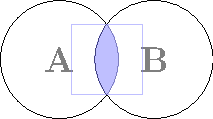
\includegraphics{../pics/set/venn2.pdf}
    \caption{Phép giao hai tập hợp}
    \label{set1}
\end{figure}

Hình \ref{set1} là biểu đồ Venn tương ứng của phép giao hai tập hợp. Khi giao của hai 
tập hợp $A$ và $B$ là rỗng thì ta nói hai tập rời nhau. Ký hiệu $A \cap B = \emptyset$.

\begin{definition}[Hợp của hai tập hợp]
    Hợp của hai tập hợp $A$ và $B$ là tập hợp các phần tử thuộc $A$ hoặc $B$.
    \begin{equation}
        A \cup B = \{ x : x \in A \text{ hoặc } x \in B \}
    \end{equation}
\end{definition}

Hình \ref{set2} là biểu đồ Venn tương ứng của phép hợp hai tập hợp.

\begin{figure}[ht]
    \centering
    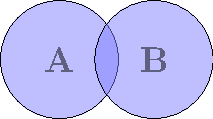
\includegraphics{../pics/set/venn3.pdf}
    \caption{Phép hợp hai tập hợp}
    \label{set2}
\end{figure}

\begin{definition}[Hiệu của hai tập hợp]
    Hợp của hai tập hợp $A$ và $B$ là tập hợp các phần tử thuộc $A$ nhưng không thuộc $B$.
    \begin{equation}
        A \backslash B = \{ x : x \in A \text{ và } x \not\in B \}
    \end{equation}
\end{definition}

Hình \ref{set3} là biểu đồ Venn tương ứng của hiệu hai tập hợp.

\begin{figure}[ht]
    \centering
    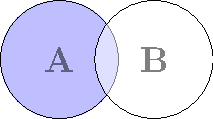
\includegraphics{../pics/set/venn4.pdf}
    \caption{Phép hiệu hai tập hợp}
    \label{set3}
\end{figure}

\section{Lực lượng của tập hợp}

Để chỉ số lượng phần tử của một tập hợp ta dùng khái niệm lực lượng của tập hợp.

Ký hiệu lực lượng của tập hợp $A$ là $\lvert A \rvert$.

Khi một tập hợp có vô số phần tử, ta gọi đó là tập vô hạn. Ngược lại ta gọi là
tập hữu hạn.

\begin{example}
    Các tập hợp số thông dụng $\NN$, $\ZZ$, $\QQ$, $\RR$ là các tập vô hạn.

    Tập hợp $A = \{ 1, 2, 3, 4, 5 \}$ là tập hữu hạn có 5 phần tử. Ký hiệu
    $\lvert A \rvert = 5$.
\end{example}

Từ biểu đồ Venn chúng ta cũng có thể tìm được công thức tính lực lượng của tập
$A \cup B$.

\begin{figure}[ht]
    \centering
    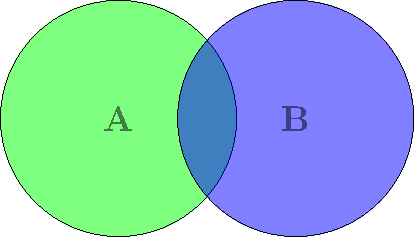
\includegraphics{../pics/set/venn1.pdf}
    \caption{Nguyên lý bù trừ cho hai tập hợp}
    \label{set4}
\end{figure}

Dựa vào hình ta có thể suy ra công thức sau

\begin{equation}
    \lvert A \cup B \rvert = \lvert A \rvert + \lvert B \rvert - \lvert A \cap B \rvert
\end{equation}

